\chapter[Ar-condicionados]{Ar-condicionados}

A termodinâmica ganhou bastante destaque desde a revolução industrial, pois seu estudo contribuiu para criação e melhoria de diferentes máquinas térmicas - principalmente máquinas a vapor - e continua tendo bastante importância no mundo moderno. Toda tecnologia que está em nossa volta teve contribuição da ciência da termodinâmica para sua criação. Por isso, mesmo que a sociedade considera as mudanças climáticas como consequência dessas tecnologias, não queremos parar de utilizá-las.

Existe uma transferência natural de energia entre corpos quentes para corpos mais frios - este fenômeno é denomidado calor. A tranferência de calor pode ocorrer por três meios distintos: radiação, convecção e condução - e se dois corpos já nâo trocam mais calor considera-se que estão em equilíbrio térmico. A troca de calor entre dois ou mais corpos podem afetar outras propriedades além da temperatura, tais como o volume e a pressão; e o ramo da física que estuda esses efeitos é a Termodinâmica \cite{Maxwell}.

O calor segue o fluxo de corpos de temperatura mais alta para os de mais baixa - fato conhecido como Segunda Lei da Termodinâmica - portanto máquinas que forçam o calor a seguir o caminho oposto ao natural, tais como geladeiras e ar-condicionados, geram sempre um custo. As máquinas térmicas em fluxo inverso (refrigeradores) foram inicialmente pensados como uma forma de calcular o rendimento máximo possível de motores térmicos por Sadi Carnot \cite{Carnot}. Porém, ar-condicionados acabaram sendo construídos sem que o seu custo em termos de aumento da entropia atmosférica fosse devidamente levado em consideração.

A analogia feita por Sadi Carnot foi comparar máquinas térmicas à uma cachoeira - sendo a fonte quente como o topo da cachoeira e a fonte fria em baixo. Desta forma é possível ver o absurdo que é querer forçar o calor a seguir um fluxo contrário ao seu natural. Por mais que seja possível fazer isso com pequenas quantidades de energia, em larga escala a cachoeira jamais irá subir com sua água. E na prática, não existe um isolamento forte entre a Fonte Quente e a Fria no caso de ar-condicionados, o que faz com que tenha um grande disperdício de energia (\autoref{carnot}).

\begin{figure}[h]
    \centering
    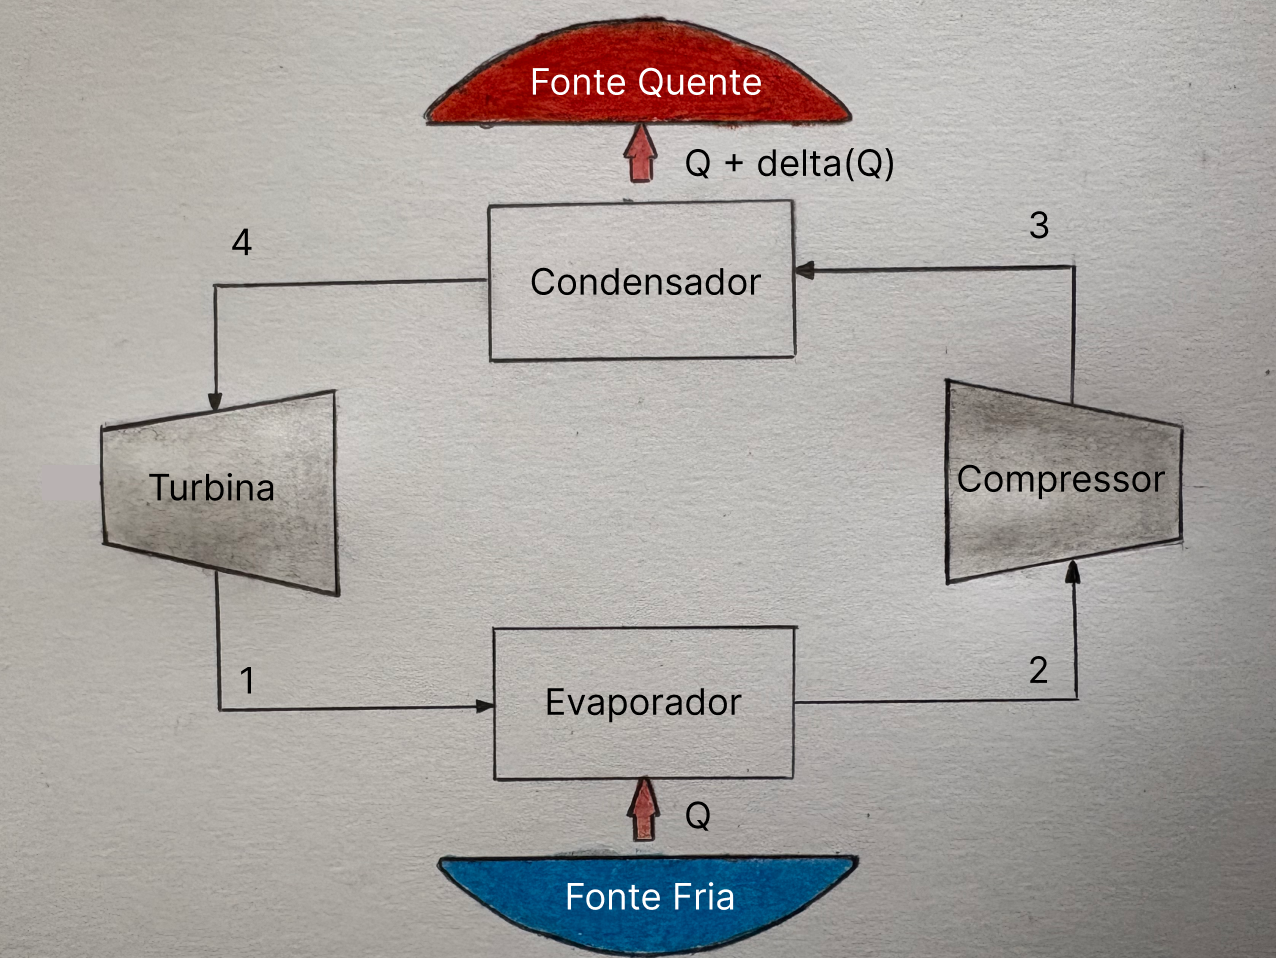
\includegraphics[scale=0.25]{pictures/carnot.png}
    \caption{Esquema do ciclo reverso de Carnot - considerado um refrigerador ideal e impossível na prática.}
    \label{carnot}
\end{figure}

Em outras palavras, ar-condicionados afetam de forma intensa a entropia da atmosfera, definido por Rudolf Clausius como a variação infinitesimal da quantidade calor pela temperatura instântanea. A entropia as vezes é denominada como medida do caos de um sistema, ou seja, se queremos estabilidade climática é essencial estar atento a máquinas que aumentam essa propriedade de forma intensa \cite{Clausius}.

O sistema de ar-condicionado simplesmente joga o calor de um cômodo para o exterior, e nesse processo parte da energia elétrica empregada é convertida em mais energia térmica. Como o calor segue seu fluxo natural, durante o período de funcionamento do ar-condicionado parte da energia térmica volta para o cômodo de origem. Além disso, como o ar quente tende a subir, o efeito é pior em casos de ACs(ar-condicionados) de andares inferiores de prédio, pois o calor eliminado irá para os apartamentos vizinhos. Nos centros urbanos estamos desperdiçando energia ao usar os ACs como método de refrigeração.

\begin{figure}[h]
    \centering
    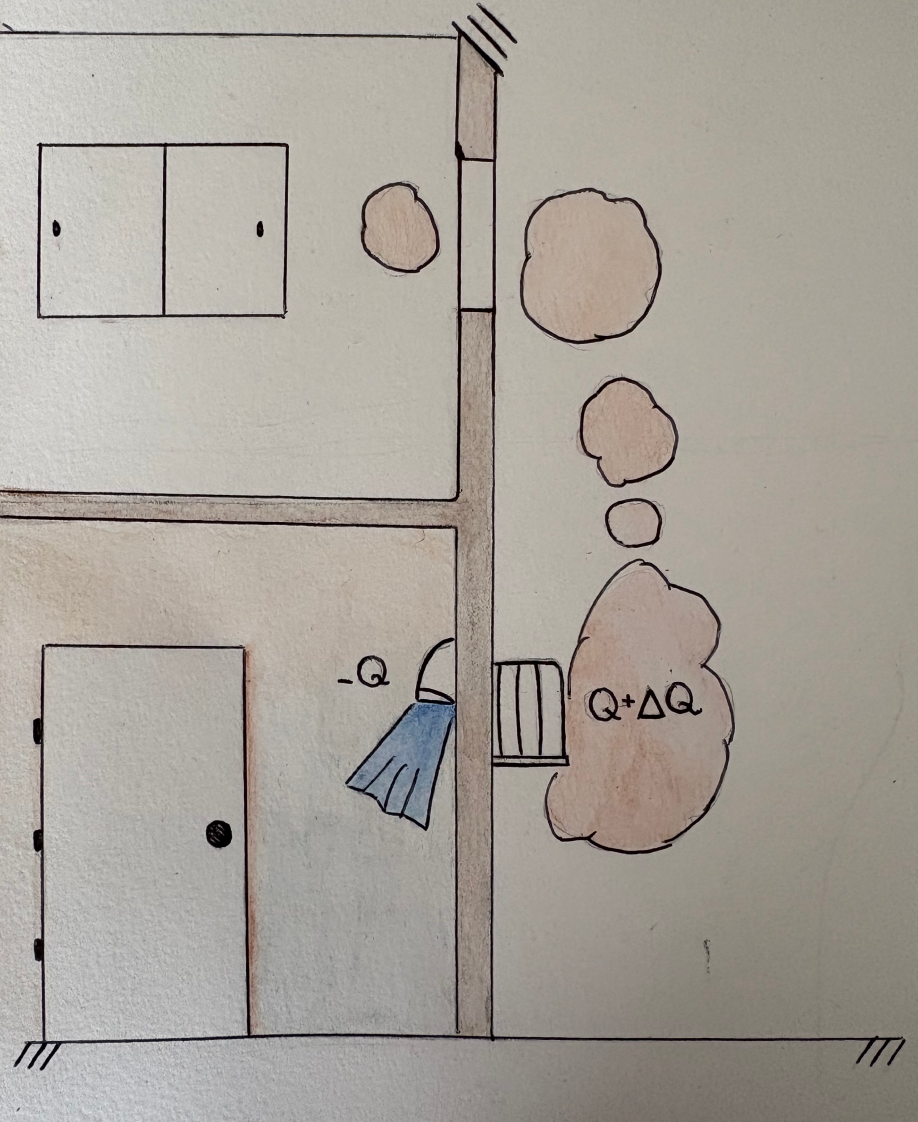
\includegraphics[scale=0.35]{pictures/predio.png}
    \caption{Ilustração do funcionamento do ar-condicionado - aumentando o calor e retornando para o ambiente de origem e apartamentos vizinhos.}
    \label{carnot}
\end{figure}

Uma analogia para o ar-condicionado é alguém retirando água com balde de um navio furado, não resolve o problema e possui um alto gasto energético, pois a água prontamente tenta retornar ao barco. Os ACs são geladeiras com portas abertas: podem aliviar o problema do calor para a pessoa imediatamente à frente, porém quando se analisa o sistema completo, sua eficiência é negativa.\textbf{ Além do mais, o Aquecimento Global é um problema público, sua solução também precisa estar na esfera da infraestrutura pública.}
                                  
Carnot em seu tratado "Reflexões sobre energia motora e fogo" tratou as máquinas térmicas de forma relativamente isolada com o ambiente. Este é um erro bem compreensível, pois na época não era possível prever que as máquinas térmicas reversas - ar-condicionado e geladeiras - seriam utilizadas em larga escala. Porém, quando deixa de analisar as máquinas de forma isolada ao ambiente, começa a se entender o problema que culminou nas mudanças climáticas que assombram a sociedade hoje em dia.                                                         

Quando se olha para uma escala global, o efeito do ar-condicionado na atmosfera é de gerar energia térmica e aumentar a entropia da atmosfera local - gerando uma zona de alta pressão - que são as ilhas de calor urbanas (\autoref{ilha-calor}). Estas máquinas não são um regriferadores de cômodos, mas sim aquecedores do mundo. A alta pressão da ilha de calor expulsa nuvens e dificulta a precipitação de chuva. Pois o ar quente precisa de mais vapor d'água para que ocorra a chuva que realmente resfriaria o ambiente urbano. Por isso, quando chove a quantidade de água é mais elevada causando tempestades, ciclones-bomba e enchentes. 

\begin{figure}[h]
    \centering
    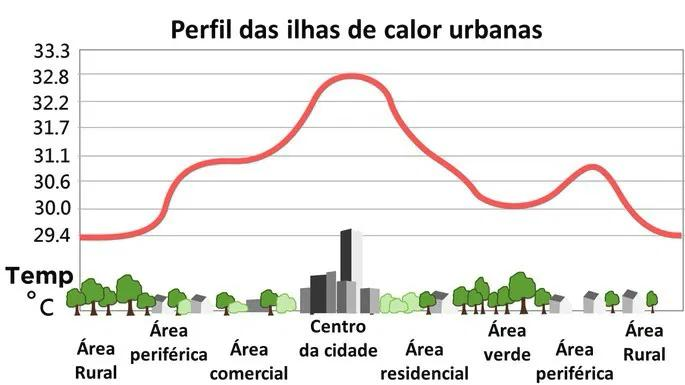
\includegraphics[scale=0.6]{pictures/ilha-calor.jpg}
    \caption{Ilustração da ilha de calor gerada pela alta queima de conbustível fóssil e refrigeração ineficiente.}
    \label{ilha-calor}
    \legend{Fonte: https://www.todamateria.com.br/ilha-de-calor/}
\end{figure}

Considerar a atmosfera como reservatório térmico com capacidade infinita é o erro que provocou o uso em larga escala do ar-condicionado. Apesar de ser verídico que a atmosfera terrestre possui grande capacidade térmica quando comparado a objetos humanos do dia-a-dia. Quando analisamos a sociedade como todo percebemos que máquinas térmicas são capazes de afetar a atmosfera em grande escala, pois estamos lidando em uma escala de centenas de milhões de ar-condicionados ao redor do mundo; e muitos deles bem concentrados em bairros específicos. 
Além disso, o ar-condicionado perde eficiência quando a temperatura externa está alta, ou seja, quando mais as pessoas têm o ímpeto de utilizar essa máquina - que são os dias quentes - menos eficiente estas serão em seu "trabalho".

                                        